\documentclass[11pt,a4paper]{article}
\usepackage{fontspec}
\usepackage{polyglossia}
\setdefaultlanguage{turkish}
\usepackage[margin=2.4cm]{geometry}
\usepackage{graphicx}
\usepackage{booktabs}
\usepackage{amsmath}
\usepackage[font=small,labelfont=bf]{caption}
\usepackage{xcolor}
\usepackage{microtype}
\usepackage[hidelinks]{hyperref}
\setlength{\emergencystretch}{3em}
\setlength{\parskip}{0.5em}
\setlength{\parindent}{0pt}
% LuaLaTeX ile derlenir (bu bilgisayarda XeLaTeX yok); XeTeX'e özgü \XeTeXinterchartokenstate gerekmez
\newcommand{\kod}[1]{\texttt{#1}}
\newcommand{\olc}{\textsc{[Ölçüldü]}}
\newcommand{\yor}{\textsc{[Yorum]}}
\newcommand{\hip}{\textsc{[Hipotez]}}

\title{Kuadrupolün manyetik merkezinin zamanla kararlılığı\\[0.3em]
\large Uzun ölçüm, 12 Kasım 2026}
\author{Hazırlayan: Claude (Anthropic) · ölçümü yöneten yazılım ve analiz}
\date{12 Kasım 2026}

\begin{document}
\maketitle

\section*{Özet}

Bugün kuadrupolün manyetik merkezinin, merkezlendikten sonra saatler içinde ne kadar kaydığını ölçtük.
Plan şuydu: önce akım yokken ortamdaki alanı ölç, sonra merkezle, bir saat akım açık ölç, bir saat akımı
kapatıp mıknatısı soğut, sonra aynı akımlarla iki saat daha ölç. Dönen bobin bu süre boyunca 8~Hz'de döndü.

Üç ana sonuç çıktı. Birincisi, akım açıkken merkez \textbf{sürekli ve tek yönde kayıyor}: x yönünde
saatte yaklaşık 30--36~µm, y yönünde saatte yaklaşık 6--7~µm. İki saatlik ölçümde bu kayma durulmadı
\olc. İkincisi, mıknatıs iki saat soğutulduktan sonra aynı akımlar verildiğinde merkez başladığı yere
\textbf{dönmedi}, kaldığı yerden devam etti \olc. Bu, kaymanın büyük kısmının basit bir ısınma olmadığını
düşündürüyor \yor. Üçüncüsü, ortamdaki alan gün boyu çok kararlıydı (en fazla 0.36~µT oynadı) ve güç
kaynaklarının akımları 1~mA'nin altında sabit kaldı; yani kaymanın kaynağı ne ortam ne de güç kaynakları
\olc. Kısa süreli ölçüm gürültüsü ise küçük: art arda gelen 10 saniyelik kayıtlar arasında yaklaşık 2~µm.

\section{Ölçüm düzeni ve gün içinde ne oldu}

Bu bölümde neyin, ne zaman ölçüldüğünü ve ölçümün neden dört parçaya bölündüğünü anlatıyoruz.

\subsection{Düzenek}
Dönen bobin (rotating coil) mıknatısın içinde 8~Hz'de döner ve gördüğü alanın harmoniklerini ölçer.
Birinci harmonik $C_1$ dipol alanıdır, ikinci harmonik $C_2$ kuadrupol alanıdır. Mıknatısın manyetik
merkezi bobinin ekseninde değilse, kuadrupol alanı bobine bir dipol gibi görünür. Merkezin bobin eksenine
göre konumu bu yüzden iki harmoniğin oranından bulunur:
\begin{equation}
  x_c + i\,y_c = -\,r_\text{ref}\,\frac{C_1 - C_1^\text{ortam}}{C_2 - C_2^\text{ortam}}
\end{equation}
Burada $r_\text{ref} = 25$~mm referans yarıçapıdır; $C_1$ ve $C_2$ tesla cinsindendir ve karmaşık
sayıdır (gerçek kısım normal, sanal kısım skew bileşen). $C^\text{ortam}$, akım yokken ölçülen alandır: Dünya'nın
ve çevredeki demirin alanı. Bunu çıkarmazsak ortam alanı da merkez kayması gibi görünür. Sonuç ($x_c$, $y_c$),
mikrometre cinsinden ``net merkez''dir.

Bir sayı örneği: bugünkü merkezlemede gradyen $G = 0.0991$~T/m çıktı. 1~µT'lik bir dipol değişimi
$1\times10^{-6}\,\text{T} \,/\, 0.0991\,\text{T/m} = 10.1$~µm merkez kaymasına karşılık gelir. Bu oranı
aşağıda sık kullanacağız.

Her 10 saniyede, o 10 saniyede alınan bütün sağlıklı ölçümlerin (tipik olarak 5 tane) ortalaması bir
``kayıt'' olarak yazıldı. Bu raporda ``akımsız'' akımların sıfır olduğu, ``akımlı'' akımların
merkezlenmiş değerlerde açık olduğu fazları anlatır.

\subsection{Zaman çizelgesi}
Ölçüm, aksaklıklar yüzünden dört parçada tamamlandı (Tablo~\ref{tab:fazlar}). Önemli olan şu: dönen bobinin
açı referansı (enkoderin sıfırı) gün boyu değişmedi. Bunu her yeniden başlangıçta akımsız ortam alanının
aynı bileşenleri verdiğini görerek doğruladık ($B_1 \approx +3.0$~µT, $A_1 \approx -33.1$~µT, farklar
0.1--0.35~µT) \olc. Bu yüzden bütün parçalar aynı koordinatta ve doğrudan karşılaştırılabilir.

\begin{table}[h]
\centering\small
\begin{tabular}{llll}
\toprule
Ad & Saat & Akımlar & Not \\
\midrule
O1 & 10:30--11:00 & sıfır & ortam, 30 dk \\
--- & 11:01 & --- & merkezleme başlarken durdu (aksaklık 1) \\
O2 & 12:00--12:05 & sıfır & ortam, 5 dk \\
--- & 12:05--12:13 & --- & merkezleme, 4 iterasyon: $x_c=-4.2$, $y_c=+4.2$~µm \\
A1 & 12:13--13:13 & açık & 9.8284 / 9.4098 / 9.1883 / 9.6069~A, 60 dk \\
O3 & 13:14--14:00 & sıfır & ortam (soğuma), ölçüm 14:00'te kesildi (aksaklık 2) \\
O4 & 15:00--15:05 & sıfır & ortam, 5 dk; ardından durdu (aksaklık 3) \\
O5 & 15:06--15:11 & sıfır & ortam, 5 dk \\
A2 & 15:12--17:12 & açık & A1 ile aynı akımlar, 120 dk \\
\bottomrule
\end{tabular}
\caption{Ölçülen fazlar. Soğuma (akımların kapalı olduğu süre) 13:13--15:12 arası, yaklaşık 2 saat.
Planlanan kapanış ortam ölçümü (20 dk) aksaklık 4 yüzünden alınamadı.}
\label{tab:fazlar}
\end{table}

\section{Ortam alanı ve güç kaynakları}

Önce kaymanın ``dışarıdan'' gelip gelmediğine bakıyoruz: ortam alanı mı değişti, yoksa güç kaynaklarının
akımı mı oynadı?

\subsection{Ortam alanı}
Akımsız fazların ortalaması gün boyu $B_1$ için 0.16~µT, $A_1$ için 0.36~µT aralığında kaldı. Bütün akımsız
kayıtlara bir doğru uydurunca gün boyu eğim $B_1$ için $+0.014 \pm 0.007$, $A_1$ için $+0.059 \pm 0.006$~µT/saat
çıkıyor \olc. Şekil~\ref{fig:ortam} bunu gösteriyor: oynamalar $\pm0.3$~µT içinde ve belirgin bir yönleri yok.

Bunu merkez cinsinden okumak için yukarıdaki oranı kullanalım: 0.36~µT, en fazla
$0.36 \times 10.1 \approx 3.6$~µm eder. Saatte 0.06~µT ise saatte yaklaşık 0.6~µm'dir. Bulduğumuz merkez kayması
(saatte 30~µm'den fazla) bunun elli katı. Yani \textbf{ortam alanı kaymayı açıklayamaz} \olc.

Dün (11 Kasım) akımsız alanda saatte ~0.95~µT'lik bir kayma görmüştük ve nedenini motorun ısınması ya da
ortam diye iki aday olarak bırakmıştık. Bugün motor sabah 30 dakika dönerken bu kadar kayma görülmedi
(O1: $B_1$ $+0.69 \pm 0.11$, $A_1$ $+0.21 \pm 0.10$~µT/saat) \olc. Dünkü kayma büyük olasılıkla o akşamki
ortama aitti \yor.

\begin{figure}[h]
\centering
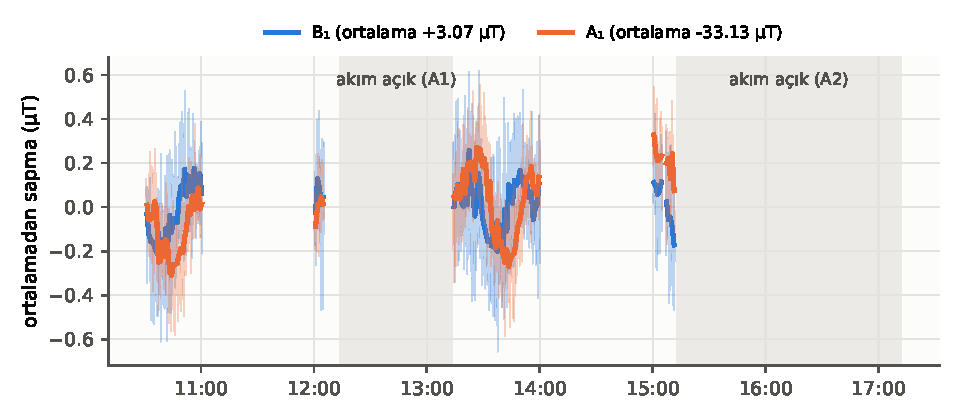
\includegraphics[width=\linewidth]{sekil1_ortam.pdf}
\caption{Akımsız fazlarda ortam dipolü, günün ortalamasından sapma. İnce çizgiler 10 s'lik kayıtlar, kalın
çizgiler 1 dakikalık ortalamalar. Gri alanlar akımların açık olduğu dönemler (orada ortam ölçülemez).}
\label{fig:ortam}
\end{figure}

\subsection{Güç kaynakları}
Akımlı fazlarda dört kaynağın ölçülen akımlarının standart sapması 0.01--0.11~mA, en büyük tepe-tepe
değişimi 0.6~mA oldu \olc. 6 Kasım raporundaki orana göre nominal akımın \%1'i (95~mA) merkezi yaklaşık
0.2~mm kaydırır; 0.6~mA bunun yüzde 0.6'sı, yani en fazla $\approx 1.3$~µm eder. \textbf{Güç kaynakları
da kaymayı açıklayamaz} \olc.

\section{Merkezin zamanla değişimi}

Bu bölüm raporun asıl sonucunu içeriyor: akım açıkken merkez nasıl hareket etti ve soğuduktan sonra ne oldu.

\subsection{Akım açıkken: sürekli kayma}
Şekil~\ref{fig:zaman} iki akımlı fazı saate göre gösteriyor. Tablo~\ref{tab:merkez} sayıları veriyor.

\begin{figure}[h]
\centering
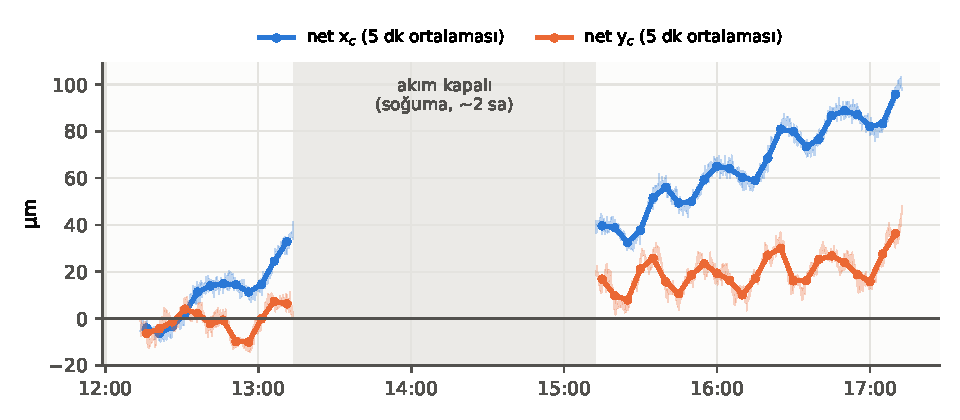
\includegraphics[width=\linewidth]{sekil4_zaman.pdf}
\caption{Net merkez, saate göre. Kalın çizgiler 5 dakikalık ortalamalar, ince çizgiler 10 s'lik kayıtlar.
Gri alan, akımların kapalı olduğu yaklaşık 2 saatlik soğuma. Akımlar yeniden açılınca merkez A1'in
başladığı yere değil, bittiği yere yakın bir yerden devam ediyor.}
\label{fig:zaman}
\end{figure}

\begin{table}[h]
\centering\small
\begin{tabular}{lrrrrr}
\toprule
 & ilk 10 dk & son 10 dk & ortalama & doğrusal eğim & ardışık kayıt \\
 & (µm) & (µm) & (µm) & (µm/saat) & gürültüsü (µm) \\
\midrule
A1, $x_c$ & $-5.3$ & $+28.6$ & $+10.5$ & $+36.4 \pm 0.9$ & 2.4 \\
A1, $y_c$ & $-5.4$ & $+6.8$ & $-1.3$ & $+6.3 \pm 1.1$ & 2.3 \\
A2, $x_c$ & $+39.2$ & $+97.5$ & $+65.3$ & $+29.8 \pm 0.4$ & 2.4 \\
A2, $y_c$ & $+13.2$ & $+48.2$ & $+19.8$ & $+6.4 \pm 0.5$ & 2.1 \\
\bottomrule
\end{tabular}
\caption{Akımlı fazlarda net merkez. Arka plan olarak hemen önceki akımsız fazın son ölçümleri çıkarıldı.
Eğimin belirsizliği yalnızca istatistiksel; gerçek hareket düz bir doğru olmadığı için asıl belirsizlik
daha büyüktür. ``Ardışık kayıt gürültüsü'' art arda iki 10~s'lik kaydın farkından hesaplanan, yavaş
kaymadan etkilenmeyen kısa süreli gürültüdür.}
\label{tab:merkez}
\end{table}

Tablodan okunanlar şunlar \olc:
\begin{itemize}
\item x yönünde iki fazda da kayma neredeyse aynı hızda: A1'de saatte 36, A2'de saatte 30~µm. A2'nin iki
saatinde x, 39~µm'den 98~µm'ye çıktı; durulma belirtisi yok.
\item y yönünde kayma daha yavaş, saatte yaklaşık 6~µm, ama 5--10 dakikalık zaman ölçeğinde $\pm10$~µm
dolaşıyor (Şekil~\ref{fig:zaman}).
\item Kısa süreli gürültü küçük ve iki fazda aynı: art arda gelen kayıtlar arasında 2.1--2.4~µm. Yani
ölçümün çözünürlüğü kaymayı rahatça görecek kadar iyi; sınırlayan şey ölçüm değil, merkezin kendi hareketi.
\end{itemize}

A1'in x eğrisi ilk 20 dakikada hızla yükselip 20--50. dakikalar arasında 13--15~µm'de yataylaşıyor, sonra
yeniden yükseliyor (Ek, Şekil~\ref{fig:x}). Bunu ilk bakışta ``ısınıp oturma'' sanmıştık; ama A2'deki
iki saatlik veri, bu yataylaşmanın geçici olduğunu gösteriyor \yor. A2'ye $x(t) = a + b\,(1 - e^{-t/\tau})$
biçiminde bir ısınma eğrisi uydurunca zaman sabiti $\tau = 255 \pm 55$~dakika çıkıyor. Bu kadar uzun bir
zaman sabiti, kaymanın iki saatte durulmasını beklememizi engelliyor; ama uydurmanın kendisi zayıf, çünkü
veri eğrinin yalnızca başını görüyor \yor.

\subsection{Soğuduktan sonra: merkez kaldığı yerden devam ediyor}
Planın asıl sorusu buydu: kayma ısınmadan geliyorsa, mıknatıs iki saat soğuyunca merkez A1'in başladığı
yere (yaklaşık $-5$~µm) dönmeli ve aynı ısınma eğrisini yeniden izlemeli.

Olan bu değil \olc. A1 x yönünde $+28.6$~µm'de bitti; iki saat sonra A2 $+39.2$~µm'de başladı. y yönünde
A1 $+6.8$~µm'de bitti, A2 $+13.2$~µm'de başladı. Aynı süreye denk gelen pencereleri karşılaştırınca
(akım açıldıktan 40--60 dakika sonra) A2 x'te 41~µm, y'de 16~µm A1'den ileride. Şekil~\ref{fig:zaman}'da
görüldüğü gibi merkez, soğuma boyunca durmuş ve akımlar açılınca kaldığı yerden yürümeye devam etmiş gibi.

\section{Yorum: kaymanın nedeni ne olabilir?}

Ölçülen olgulardan dışarıda kalan ama anlamaya yardım eden yorumlarımızı burada topluyoruz.

\textbf{Ortam ve güç kaynakları dışlandı} \olc. İkisinin katkısı en fazla birkaç µm; kayma ise onlarca µm (A2'nin iki saatinde yaklaşık 60~µm).

\textbf{Saf ısınma zayıf bir açıklama} \yor. Isınma olsaydı soğuyunca geri dönmesini beklerdik. Dönmedi.
Bir ihtimal, ısıl zaman sabitinin soğumada da birkaç saat olması: o zaman iki saatlik soğuma merkezi geri
getirmeye yetmemiş olabilir. Ama A2'deki kaymanın hızı A1'dekiyle neredeyse aynı (30 ve 36~µm/saat);
mıknatıs A1'in sonundaki sıcaklığından biraz soğumuş olsaydı A2'nin başında daha hızlı bir yükseliş
görürdük. Görmüyoruz.

\textbf{Mekanik sünme (yavaş kayma) güçlü bir aday} \hip. Bobinin ya da milin mıknatısa göre konumu yavaşça
değişiyorsa, merkez bobin eksenine göre kayıyormuş gibi görünür. Bu kayma akımdan bağımsız olduğu için
akımsız fazlarda da sürer, ama orada göremeyiz: ortam alanı düzgün olduğu için bobinin yanal konumu
ortam ölçümüne iz bırakmaz. Bu açıklama üç gözlemle uyumlu:
\begin{itemize}
\item Soğumadan sonra merkez kaldığı yerden devam etti (sünme soğumada da sürmüş olabilir).
\item Sabahki kısa denemedeki merkezlemeyle (10:20) öğlenki merkezleme (12:13) arasında akımlar 4--20~mA
farklı çıktı; bu da iki saatte birkaç on µm'lik bir kaymaya karşılık gelir \olc.
\item Dün şaft kaydırıldı ve mile kütle eklendi; ayrıca milde 19.7~Hz'de bir titreşim var. Yeni ayarlanmış
bir mekanik düzenin titreşim altında yavaşça oturması akla yatkın \hip.
\end{itemize}

\textbf{Nasıl ayırt edilir} \yor. Mekanik sünmeyi doğrudan görmek için akımlar açıkken bobini durdurmadan
uzun süre izlemek ve ara sıra mili bir referansa göre ölçmek gerekir. Daha basit bir test: akımlar kapalıyken
bobini bir saat döndürüp hemen kısa bir merkezleme yapmak. Merkez yine kaymışsa, kayma akımdan ve ısınmadan
bağımsızdır.

\section{Aksaklıklar ve düzeltmeler}

Ölçümün dört parçada tamamlanmasına yol açan aksaklıklar ve yapılan düzeltmeler şunlardır.

\begin{enumerate}
\item \textbf{11:01, güç kaynağı yanıt kayması.} Merkezleme başlarken bir güç kaynağına giden sorgular
bir önceki sorgunun yanıtını almaya başladı; program bunu cihaz hatası sayıp akımları güvenle sıfırladı.
Önce bunun 2~s'lik zaman aşımından geldiğini sandım; bu yanlıştı. Kayıtlarda hiçbir sorgu 2~s'ye
yaklaşmıyor. Kayma, iki iş parçacığı farklı kaynaklara aynı anda sorgu göndermeye başlayınca başladı.
Düzeltme: bütün kaynaklar için tek ortak iletişim kilidi; ayrıca tampon boşaltma ve yanıt biçimi denetimi.
Sonraki merkezlemelerde kayma görülmedi.
\item \textbf{14:00, ölçüm dışarıdan durduruldu.} Ölçüm, Claude Code'un arka plan görevlerine koyduğu 2 saatlik
sınıra takıldı. Kapanış kodu çalışmadı (akımlar o sırada zaten sıfırdı). Düzeltme: sonraki ölçümler ayrı bir
sistem servisi olarak çalıştırıldı; betik artık SIGTERM'de de akımları rampayla sıfırlıyor.
\item \textbf{15:05, devam ederken yazılım hatası.} Merkezlemeyi atlayıp verilen akımlarla devam etme
seçeneği güç kaynaklarını başlatmayı unutuyordu. Akım verilmeden güvenle durdu, düzeltildi.
\item \textbf{16:55, USB bağlantısı parazitten koptu.} Sistem günlüğünde ``\kod{usb 3-2-port1: disabled by hub
(EMI?)}'' görüldü. 0004 numaralı kaynak yeniden bağlandı ama çalışan program eski bağlantıyı kullandığı için
onu artık kontrol edemedi. Kaynağın çıkışı ayarlı akımda kaldı (sonradan 9.6073~A okundu, ayar 9.6069~A), yani
A2'nin son 17 dakikası da geçerli \olc. Ancak 17:12'de program akımları sıfırlayamadı; akımlar, kullanıcının
Telegram'dan verdiği onayla yeni bağlantılarla rampayla sıfırlandı ve çıkışlar kapatıldı. Planlanan kapanış
ortam ölçümü (20~dk) bu yüzden alınamadı. A2'nin son 10 dakikasında y'deki sıçramanın ($+31.7 \rightarrow
+48.2$~µm) bu olayla ilgisi olup olmadığını bilmiyoruz \hip.
\end{enumerate}

Bu sırada ortaya çıkan bir genel öneri: uzun ölçümlerde güç kaynaklarının USB kabloları ve hub, motor
sürücüsü ve kayar halka gibi parazit kaynaklarından uzak tutulmalı; program kopan bir kaynağa
kendiliğinden yeniden bağlanabilmeli.

\section{Sonuç ve öneriler}

Bugünkü ölçüm, merkezleme düzeneğinin kısa süreli çözünürlüğünün çok iyi olduğunu (10 saniyede ~2~µm)
ama merkezin saatler içinde onlarca µm kaydığını gösterdi. 5~µm'lik bir merkezleme hedefi için bu kayma
belirleyici: merkezleme bittikten birkaç dakika sonra merkez toleransın dışına çıkıyor.

Önerilerimiz:
\begin{enumerate}
\item \textbf{Kaymanın mekanik mi ısıl mı olduğunu ayırmak} için Bölüm~4'teki basit testi yapmak: akımlar
kapalıyken bobini bir saat döndürmek, sonra kısa bir merkezleme yapmak.
\item \textbf{Mekanik düzeni sabitlemek:} şaft ve kütle dün ayarlandığı için düzenin oturmasını beklemek ya da
bağlantıları sıkılaştırmak, sonra ölçümü tekrarlamak.
\item \textbf{Kapanış ortam ölçümünü} bir sonraki uzun ölçümde mutlaka almak (bugün kaçtı).
\item Uzun ölçümleri ayrı bir servis olarak çalıştırmayı ve USB kaynaklarına yeniden bağlanmayı kalıcı hale getirmek.
\end{enumerate}

\appendix
\section{Ek: akım açıldıktan sonra geçen süreye göre}
Aşağıdaki şekiller iki akımlı fazı, akımlar açıldıktan sonra geçen süreye göre üst üste koyuyor. Isınma
olsaydı iki eğri birbirini izlemeliydi; aralarındaki fark, soğumada geri dönmeyen kaymadır.

\begin{figure}[h]
\centering
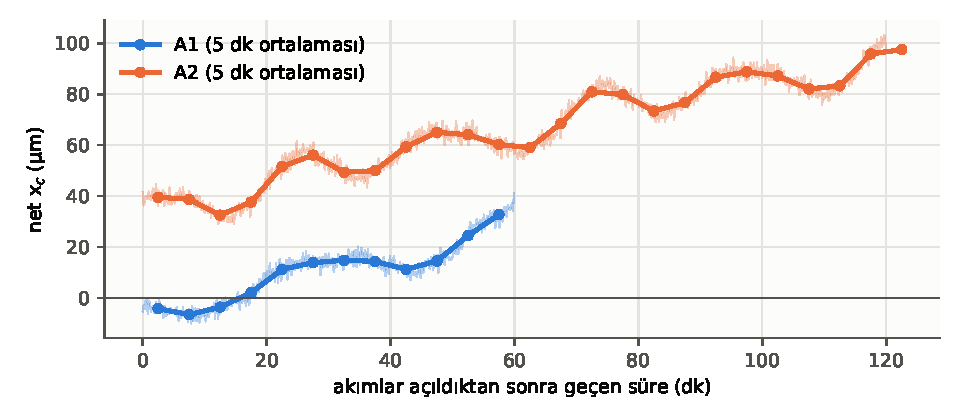
\includegraphics[width=\linewidth]{sekil2_x.pdf}
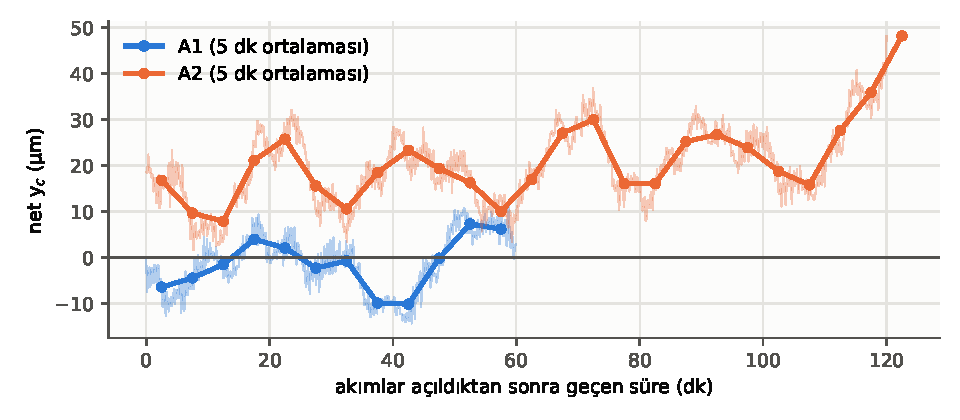
\includegraphics[width=\linewidth]{sekil3_y.pdf}
\caption{Net $x_c$ (üstte) ve $y_c$ (altta), akımlar açıldıktan sonra geçen süreye göre. Kalın çizgiler
5 dakikalık ortalamalar.}
\label{fig:x}
\end{figure}

\vfill
{\small Veriler: \kod{kayitlar/2026-11-12\_103042}, \kod{\_120020}, \kod{\_150000}, \kod{\_150645};
sağlam kısımlar ve notlar \kod{kayitlar/uzun\_kararlilik\_2026-11-12/}. Analiz:
\kod{donen\_bobin/host/uzun\_kararlilik\_analiz.py}; bütün sayılar \kod{rapor/sonuclar.json}'dan.}

\end{document}
